\section{Model and Goals}
\label{sec:model}
In this section we describe our system actors, our threat model and our design goals.

\subsection{Actors}
\label{sec:model:actors}
The main actors in our scheme are the log server, which appends statements to the log, \Sys clients, which verify new statements and check for non-equivocation, and the header relay network (HRN), which helps scale \Sys to support a large number of clients (see \figref{fig:communication}).

\subsubsection{Log server}
\label{sec:model:actors:log-server}
A log server manages an append-only log of application-specific \emph{statements}.
The log server appends statements to the log by signing Bitcoin transactions with statement data embedded in them and broadcasting them to the Bitcoin P2P network.
We call these transactions \emph{\Sys transactions} and defer their discussion to \secref{sec:catena:design:transactions}.
In this paper, we will mostly talk about a single log server managing the log, but by using Bitcoin multisignatures\cite{multisig}, \Sys can support multiple servers who either jointly or separately append statements to the log.
Also, although a log server can manage many different logs, for simplicity we restrain our discussion to a single server managing a single log.

\subsubsection{Clients}
Multiple clients connect to the log server and keep up with new log statements.
As depicted in \figref{fig:communication}, clients fetch \Sys transactions from the log server and verify they have been included in the Bitcoin blockchain.
This verification is done against block headers obtained from the header relay network (discussed next).
\Sys clients want to prevent log server equivocation: a client who is shown a statement $s_i$ wants to ensure there is no other contradictory statement $s_i'$ in the log at position $i$ (see \secref{sec:model:goals:noneq}).

\subsubsection{Header Relay Network}
Due to the low connection capacity of the Bitcoin P2P network (see \secref{sec:catena:design:header-relay}), \Sys clients use a separate header relay network (HRN) to obtain Bitcoin block headers (see \secref{sec:catena:design:header-relay}).
Otherwise, \Sys would put unnecessary stress on Bitcoin's P2P network and would not scale well.

\newcommand{\api}{\hangindent=\parindent \hangafter=1 \noindent}
\newcommand{\createlog}{\mathsf{CreateLog}\xspace}
\newcommand{\appendstmt}{\mathsf{AppendStmt}\xspace}
\newcommand{\verifystmt}{\mathsf{VerifyStmt}\xspace}
\newcommand{\txgen}{\mathsf{tx}_{\textsf{genesis}}}

\subsection{\Sys API}
\label{sec:model:api}

Our scheme can be succinctly described as a tuple $\langle \createlog, \appendstmt, \verifystmt \rangle$ of API calls.
For clarity, we prefix calls with $S$ when they are made by the log server and with $C$ when they are made by clients.
\\

\api $S.\createlog(d) \rightarrow (\sK, \pK)$.
Creates an empty log. 
All future log statements can be verified against the log's public key $\pK$.
Embeds some arbitrary data $d$ in the log (e.g., the log's name).

\api $S.\appendstmt(\sK, s_i)$.
Appends the statement $s_i$ to the log, signing it using $\sK$.

\api $C.\verifystmt(\pK, i, s_i) \rightarrow \{\mathsf{True, False}\}$.
Verifies that the statement $s_i$ is contained in the log with \pk $\pK$ at position $i$.
Returns true if successful or false otherwise.
Before being called on $s_i$, $\verifystmt$ must first be called on $s_1, s_2, \dots, s_{i-1}$, in that order.
\\

To recap, a server creates a new log by calling $\createlog$ and appends statements to this log using $\appendstmt$.
Clients verify each new statement $s_i$ by calling $\verifystmt$ in order for $i = 1, 2, 3, \cdots$.

\subsection{Threat Model}
\label{sec:catena:threat-model}
% Previous work assumptions:
% .CT: Not stated specifically, but they assume STH-gossiping, trusted monitors and trusted auditors.
% .ECT: Malicious-but-cautious; can mount active attacks but only if he stays undetected. One assumption seems to be the adversary cannot equivocate because gossiping will detect it.
% .CONIKS: Does not mention anything about "network", "active" or "passive" adversaries. Assumes a PKI for providers. Providers can deter each other from equivocating.
% .AKI: CAs, public logs and validators do not collude. Browsers have their PKs (like a small PKI). Adversary can gain control of some but not all the servers the user trusts. Adversary can gain control of all servers that the user does NOT trust.
% .ARPKI: Active adversary can drop, modify, insert messages at will (to a certain extent), but he cannot compromise keys of certain actors (only n-1 out of n can be compromised).

% Server can equivocate
% ---------------------
\subsubsection{Adversarial Log Server}
\label{sec:model:threat:log-server}
We assume the \Sys log server is compromised or coerced and wants to equivocate about statements.
We assume \Sys clients can correctly obtain the log's genesis transaction which acts as the log's ``public key'' (see \secref{sec:catena:design:genesis}).
We note that both \Sys and previous work\cite{ct,ect,coniks,aki,arpki,cosi} all rely on some sort of initial public-key distribution.
However, unlike previous work, \Sys can prevent equivocation once a client has the ``public key'' or genesis transaction.
It's important to understand that, similarly to how a signature can only be verified with respect to a public key, equivocation can only be prevented with respect to a log identified by some kind of information, in this case, the genesis transaction.

We stress that \Sys's goal is to prevent equivocation given a log's genesis transaction and orthogonal techniques can be used for distributing the genesis transaction.
For instance, the log's genesis transaction can be shipped with the application software that audits that log, similar to how browsers are shipped with public keys of Certificate Authorities (CAs).
In fact, we argue it might be easier for end-users to verify the genesis transaction if they know the log's creation date.
Specifically, users can download just the blocks around that date and check that no other genesis transaction for the log exists in those blocks.

% Proof-of-work consensus
% -----------------------
\subsubsection{Proof-of-Work Consensus}
\label{sec:model:threat:pow}
Similar to previous work \cite{virtualchain, blockstack, keybase, bitcoin-smc, bitcoin-anon-cred, versum, bitcoin-incent-comp, bitcoin-pred-mkt,commitcoin}, we assume that adversaries cannot break Bitcoin's proof-of-work consensus and fork the blockchain.
Specifically, we assume that a \Sys transaction is immutable once it has been confirmed by a sufficient number of blocks, as configured by \Sys clients individually (we recommend at least 6 blocks).
We believe it is reasonable to assume that long malicious forks are unlikely to occur due to the computational difficulty and financial burden of such an attack.
We also assume the \Sys log server cannot collude with large Bitcoin miners, who are not likely to benefit financially from a forking attack.
Finally, we have to assume Bitcoin's P2P network is reliable and miners hear about each other's blocks quickly, or else proof-of-work consensus could be easily subverted\cite{blockchainproto,eclipse}.
We discuss attacks on Bitcoin's consensus in more detail in \secref{sec:attacks}.


% or t for top, b for bottom, h for here (https://tex.stackexchange.com/questions/35125/how-to-use-the-placement-options-t-h-with-figures)
\begin{figure}[t]
    \centering
    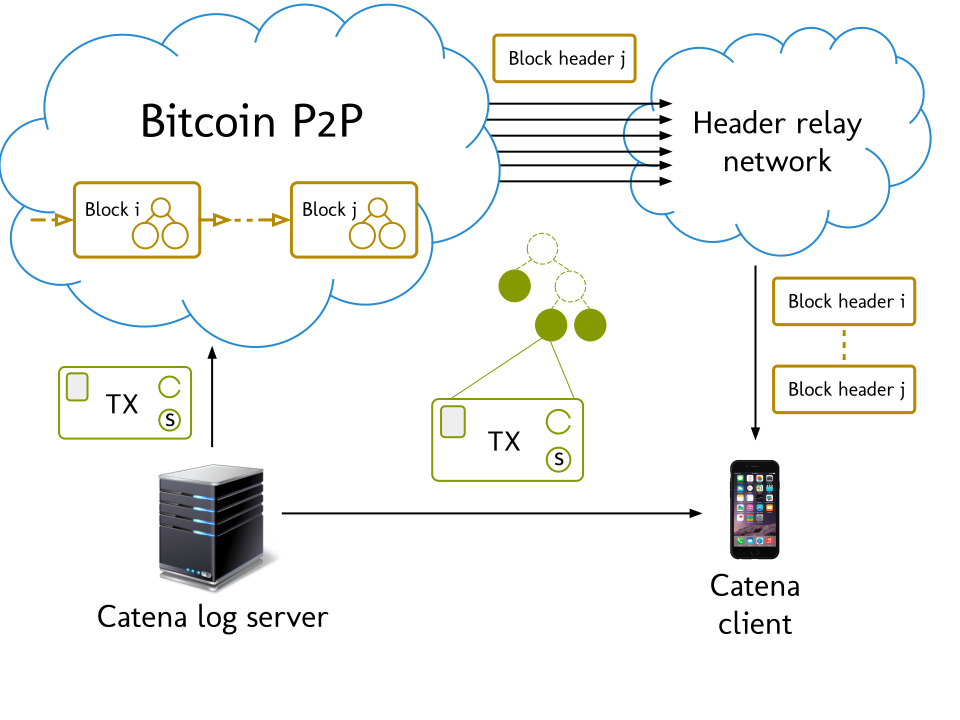
\includegraphics[width=1\columnwidth]{figs/communication.eps}
    \vspace{-1.2cm}
    \caption{The log server broadcasts \Sys transactions with statements embedded in them to the Bitcoin P2P network. \Sys clients query the header relay network for block headers and the log server for statements with proofs they were witnessed in the Bitcoin blockchain. The header relay network maintains good connectivity to the Bitcoin P2P network without depleting the P2P network's connection pool.}
    \label{fig:communication}
\end{figure}

% Thin client assumption
% ----------------------
\subsubsection{SPV Assumption}
\Sys clients use thin nodes (see \secref{sec:background:bitcoin:thin}) to efficiently verify the log for non-equivocation.
It's important to note that thin nodes are less secure than full nodes against adversarial mining attacks (see \secref{sec:attacks:adversarial-mining}).
Also, thin nodes have to assume miners verify their own blocks and the blocks of other miners before mining, otherwise thin nodes risk accepting invalid transactions.
Fortunately, Bitcoin miners have a strong incentive to verify blocks, as they would lose the block reward if they extend an invalid blockchain.
However, recent work\cite{consensuscomputer} shows that when block verification is expensive miners have an incentive to skip it.
We discuss such an event that occurred in 2015 in \secref{sec:attacks:accidental-forks}.

\subsubsection{Header Relay Network}
% This network is open => Sybil attacks => eclipse attacks => easier generalized Vector76 attacks / Finney attacks (but we discuss defenses later)
% This network is NOT open => contradicts our motivation about requiring trustworthy parties to come into existence
We trust \Sys's header relay network to serve \Sys clients with the latest Bitcoin block headers.
Similar to a compromised Bitcoin P2P network, a compromised HRN can eclipse\cite{eclipse} \Sys clients and help adversaries win mining races faster and thus equivocate (see \secref{sec:attacks:adversarial-mining}).
However, such adversaries would need a significant fraction of mining power to win races fast enough without \Sys clients noticing they are being eclipsed.
We discuss such attacks in \secref{sec:attacks:hrn}.

\subsection{Goals}
\label{sec:catena:goals}
Our goals are to prevent equivocation and to do so in an efficiently-verifiable manner, enabling each user to audit individually and thus minimizing trust in applications such as \pkds.

\subsubsection{Non-equivocation}
\label{sec:model:goals:noneq}
A log server should have a hard time equivocating about log statements.
\Sys makes equivocation in the log as hard as forking the Bitcoin blockchain, which we believe to be a reasonable amount of protection for many applications, including \pkds.
If our assumptions are broken and the Bitcoin blockchain forks, \Sys cannot prevent equivocation but still makes equivocation detectable once the forks are resolved, similar to previous gossip-based approaches\cite{ctgossip,ect,coniks,dtki}.

% Clarification about why equivocation is problematic
% ---------------------------------------------------
It's important to understand what non-equivocation actually provides.
Non-equivocation does not prevent the adversarial log server from issuing incorrect statements that break semantics at the application layer.
Instead, non-equivocation simply guarantees that all clients see all issued statements, including incorrect ones.
This allows clients to detect attacks at the application layer, as we discuss later in \secref{sec:discussion:agnostic}.

\subsubsection{Publicly Verifiable}
Given a log's genesis transaction $\txgen$ (i.e., its \pk), anyone can verify the full history of statements in that log.
Specifically, a client can obtain all statements $\langle s_1, s_2, \dots, s_n \rangle$ in the log and verify them with respect to $\txgen$.
Verification here means that a statement is part of the log at some position $i$ and no other inconsistent statement at position $i$ exists (\ie non-equivocation).
In particular, for any statement $s_i$, the log server gives the client a publicly verifiable proof $p$ with respect to the log's $\txgen$ that proves that $s_i$ is indeed the only statement in the log at position $i$.

\subsubsection{Efficiently Verifiable}
\label{sec:catena:goals:efficiency}
\Sys clients should be able to audit logs efficiently without downloading the entire Bitcoin blockchain.
Recent blockchain-based transparency work\cite{keybase,blockstack,coniks} is inefficient, requiring auditors to download the entire blockchain to prevent equivocation (see \secref{sec:background:motivation:blockchain-transparency}).
This raises the barrier to entry for log auditors, who might have to outsource auditing or trust the log blindly.
In contrast, the barrier for \Sys clients is very low: clients only download 80-byte block headers for each Bitcoin block and 600-byte Merkle membership proofs for each statement (see \secref{sec:catena:design:auditing}).
